% GENERATED by manuscript/Preprint/make_preprint.py from the manuscript sources. Do not edit by hand.
\documentclass{article}
\usepackage{arxiv}
\usepackage[utf8]{inputenc}
\usepackage[T1]{fontenc}
\usepackage{hyperref}
\usepackage{xurl}
\usepackage{amsmath,amssymb}
\usepackage{microtype}
\usepackage{graphicx}
\usepackage[numbers,sort&compress,merge,round]{natbib}
\usepackage{jabbrv}
\usepackage{authblk}
\usepackage[labelfont=bf,labelsep=period,font=small]{caption}
\captionsetup[figure]{name=Fig.}
\usepackage{titlesec}
\renewcommand\Authfont{\bfseries}
\setlength{\affilsep}{0.3em}
\graphicspath{{../}}
\urlstyle{same}
% run-in subheadings, references numbered "1." in a smaller font
\titleformat{\subsection}[runin]{\normalsize\bfseries}{}{0pt}{}[.]
\titlespacing*{\subsection}{0pt}{1.2ex plus 0.4ex minus 0.2ex}{0.5em}
\renewcommand{\bibnumfmt}[1]{#1.}
\renewcommand{\bibfont}{\small}
\setlength{\bibsep}{0.15ex plus 0.1ex}

% BEGIN NUMBERS (generated by modeling/make_numbers.py; do not edit by hand)
\newcommand{\NCatalogue}{452}
\newcommand{\CatalogueDate}{5 November 2026}
\newcommand{\NDistinct}{344}
\newcommand{\NIncluded}{249}
\newcommand{\NRuns}{five}
\newcommand{\NConditions}{666}
\newcommand{\NCalls}{3,330}
\newcommand{\NValid}{3,220}
\newcommand{\PctValid}{96.7\%}
\newcommand{\NValidAnalysed}{3,210}
\newcommand{\CollectionDate}{6 November 2026}
\newcommand{\TotalCost}{35}
\newcommand{\MaxTokens}{32{,}768}
\newcommand{\NAnalysed}{241}
\newcommand{\NDevelopers}{33}
\newcommand{\NUS}{118}
\newcommand{\NChina}{99}
\newcommand{\NOther}{24}
\newcommand{\NExcluded}{8}
\newcommand{\NNoValid}{6}
\newcommand{\NNoRegion}{2}
\newcommand{\NRegionAddedDevelopers}{2}
\newcommand{\NRegionAddedModels}{3}
\newcommand{\NFree}{2}
\newcommand{\NCells}{649}
\newcommand{\NMultiLevel}{168}
\newcommand{\NCompleteRuns}{627}
\newcommand{\LLMMean}{10.2\%}
\newcommand{\LLMMedian}{10.0\%}
\newcommand{\LLMSD}{4.6}
\newcommand{\LLMIQR}{7.3--13.0\%}
\newcommand{\LLMShareFiveFifteen}{84\%}
\newcommand{\LLMShareQuarter}{0\%}
\newcommand{\LLMPctFive}{3.5\%}
\newcommand{\LLMPctNinetyFive}{15.8\%}
\newcommand{\HumanMean}{16.2\%}
\newcommand{\HumanMedian}{5\%}
\newcommand{\HumanSD}{23.0}
\newcommand{\HumanIQR}{1.0--20.0\%}
\newcommand{\HumanShareFiveFifteen}{30\%}
\newcommand{\HumanShareQuarter}{22\%}
\newcommand{\HumanPctFive}{0\%}
\newcommand{\HumanPctNinetyFive}{70\%}
\newcommand{\NHuman}{1,321}
\newcommand{\HumanShareZero}{15\%}
\newcommand{\HumanShareHalf}{14\%}
\newcommand{\LLMNQuarter}{one}
\newcommand{\LLMRound}{10\%}
\newcommand{\LLMMin}{0.01\%}
\newcommand{\LLMMax}{42\%}
\newcommand{\SDRatio}{5}
\newcommand{\PVarTest}{$P < 0.001$}
\newcommand{\MeanUS}{10.2\%}
\newcommand{\MeanChina}{10.3\%}
\newcommand{\MeanOther}{10.4\%}
\newcommand{\ShareCiteExperts}{18\%}
\newcommand{\PrecisionRatioDate}{2.43}
\newcommand{\CIPrecisionRatioDate}{1.84--3.21}
\newcommand{\PPrecisionRatioDate}{$P < 0.001$}
\newcommand{\MedianRelease}{5 March 2026}
\newcommand{\SDBeforeMedian}{5.5}
\newcommand{\SDFromMedian}{3.4}
\newcommand{\NBeforeMedian}{119}
\newcommand{\NFromMedian}{122}
\newcommand{\ORPriceEst}{1.29}
\newcommand{\CIPriceEst}{1.16--1.43}
\newcommand{\PPriceEst}{$P < 0.001$}
\newcommand{\ORDateEst}{1.06}
\newcommand{\CIDateEst}{0.92--1.22}
\newcommand{\PDateEst}{$P = 0.42$}
\newcommand{\ORChinaEst}{1.25}
\newcommand{\CIChinaEst}{1.03--1.52}
\newcommand{\PChinaEst}{$P = 0.023$}
\newcommand{\OROtherEst}{1.02}
\newcommand{\CIOtherEst}{0.78--1.33}
\newcommand{\POtherEst}{$P = 0.89$}
\newcommand{\ORContextEst}{0.89}
\newcommand{\CIContextEst}{0.72--1.10}
\newcommand{\PContextEst}{$P = 0.30$}
\newcommand{\OROpenEst}{0.98}
\newcommand{\CIOpenEst}{0.83--1.17}
\newcommand{\POpenEst}{$P = 0.85$}
\newcommand{\ORNoneEst}{1.05}
\newcommand{\CINoneEst}{1.00--1.11}
\newcommand{\PNoneEst}{$P = 0.062$}
\newcommand{\ORXhighEst}{1.06}
\newcommand{\CIXhighEst}{0.98--1.14}
\newcommand{\PXhighEst}{$P = 0.12$}
\newcommand{\ORMaxEst}{1.07}
\newcommand{\CIMaxEst}{0.99--1.15}
\newcommand{\PMaxEst}{$P = 0.11$}
\newcommand{\ORPriceUB}{1.49}
\newcommand{\CIPriceUB}{1.35--1.65}
\newcommand{\PPriceUB}{$P < 0.001$}
\newcommand{\ORDateUB}{1.21}
\newcommand{\CIDateUB}{1.05--1.38}
\newcommand{\PDateUB}{$P = 0.007$}
\newcommand{\ORChinaUB}{1.38}
\newcommand{\CIChinaUB}{1.14--1.69}
\newcommand{\PChinaUB}{$P = 0.001$}
\newcommand{\OROtherUB}{1.07}
\newcommand{\CIOtherUB}{0.80--1.43}
\newcommand{\POtherUB}{$P = 0.66$}
\newcommand{\ORContextUB}{1.06}
\newcommand{\CIContextUB}{0.86--1.30}
\newcommand{\PContextUB}{$P = 0.61$}
\newcommand{\OROpenUB}{1.02}
\newcommand{\CIOpenUB}{0.86--1.20}
\newcommand{\POpenUB}{$P = 0.86$}
\newcommand{\ORNoneUB}{0.93}
\newcommand{\CINoneUB}{0.88--0.98}
\newcommand{\PNoneUB}{$P = 0.006$}
\newcommand{\ORXhighUB}{1.11}
\newcommand{\CIXhighUB}{1.03--1.20}
\newcommand{\PXhighUB}{$P = 0.004$}
\newcommand{\ORMaxUB}{1.14}
\newcommand{\CIMaxUB}{1.05--1.23}
\newcommand{\PMaxUB}{$P = 0.001$}
\newcommand{\ORPriceLB}{1.13}
\newcommand{\CIPriceLB}{1.00--1.27}
\newcommand{\PPriceLB}{$P = 0.050$}
\newcommand{\ORDateLB}{0.93}
\newcommand{\CIDateLB}{0.78--1.10}
\newcommand{\PDateLB}{$P = 0.38$}
\newcommand{\ORChinaLB}{1.23}
\newcommand{\CIChinaLB}{0.99--1.52}
\newcommand{\PChinaLB}{$P = 0.060$}
\newcommand{\OROtherLB}{1.02}
\newcommand{\CIOtherLB}{0.75--1.38}
\newcommand{\POtherLB}{$P = 0.90$}
\newcommand{\ORContextLB}{0.78}
\newcommand{\CIContextLB}{0.60--1.00}
\newcommand{\PContextLB}{$P = 0.049$}
\newcommand{\OROpenLB}{0.97}
\newcommand{\CIOpenLB}{0.79--1.18}
\newcommand{\POpenLB}{$P = 0.74$}
\newcommand{\ORNoneLB}{1.24}
\newcommand{\CINoneLB}{1.15--1.34}
\newcommand{\PNoneLB}{$P < 0.001$}
\newcommand{\ORXhighLB}{1.03}
\newcommand{\CIXhighLB}{0.91--1.16}
\newcommand{\PXhighLB}{$P = 0.65$}
\newcommand{\ORMaxLB}{1.06}
\newcommand{\CIMaxLB}{0.93--1.20}
\newcommand{\PMaxLB}{$P = 0.39$}
\newcommand{\ORPriceRogue}{1.59}
\newcommand{\CIPriceRogue}{0.93--2.73}
\newcommand{\PPriceRogue}{$P = 0.089$}
\newcommand{\ORDateRogue}{0.48}
\newcommand{\CIDateRogue}{0.22--1.04}
\newcommand{\PDateRogue}{$P = 0.063$}
\newcommand{\ORChinaRogue}{0.87}
\newcommand{\CIChinaRogue}{0.31--2.44}
\newcommand{\PChinaRogue}{$P = 0.79$}
\newcommand{\OROtherRogue}{1.43}
\newcommand{\CIOtherRogue}{0.28--7.33}
\newcommand{\POtherRogue}{$P = 0.67$}
\newcommand{\ORContextRogue}{1.37}
\newcommand{\CIContextRogue}{0.44--4.28}
\newcommand{\PContextRogue}{$P = 0.59$}
\newcommand{\OROpenRogue}{1.69}
\newcommand{\CIOpenRogue}{0.67--4.24}
\newcommand{\POpenRogue}{$P = 0.26$}
\newcommand{\ORNoneRogue}{0.98}
\newcommand{\CINoneRogue}{0.66--1.44}
\newcommand{\PNoneRogue}{$P = 0.91$}
\newcommand{\ORXhighRogue}{1.80}
\newcommand{\CIXhighRogue}{0.99--3.28}
\newcommand{\PXhighRogue}{$P = 0.054$}
\newcommand{\ORMaxRogue}{10.44}
\newcommand{\CIMaxRogue}{4.44--24.55}
\newcommand{\PMaxRogue}{$P < 0.001$}
\newcommand{\ORWithinEst}{1.00}
\newcommand{\CIWithinEst}{0.99--1.01}
\newcommand{\PWithinEst}{$P = 0.96$}
\newcommand{\ORBetweenEst}{0.98}
\newcommand{\CIBetweenEst}{0.90--1.07}
\newcommand{\PBetweenEst}{$P = 0.61$}
\newcommand{\ORWithinUB}{1.03}
\newcommand{\CIWithinUB}{1.02--1.04}
\newcommand{\PWithinUB}{$P < 0.001$}
\newcommand{\ORBetweenUB}{1.03}
\newcommand{\CIBetweenUB}{0.94--1.11}
\newcommand{\PBetweenUB}{$P = 0.56$}
\newcommand{\ORWithinLB}{0.96}
\newcommand{\CIWithinLB}{0.95--0.98}
\newcommand{\PWithinLB}{$P < 0.001$}
\newcommand{\ORBetweenLB}{0.88}
\newcommand{\CIBetweenLB}{0.79--0.97}
\newcommand{\PBetweenLB}{$P = 0.011$}
\newcommand{\ORWithinRogue}{1.23}
\newcommand{\CIWithinRogue}{1.13--1.34}
\newcommand{\PWithinRogue}{$P < 0.001$}
\newcommand{\ORBetweenRogue}{0.69}
\newcommand{\CIBetweenRogue}{0.44--1.09}
\newcommand{\PBetweenRogue}{$P = 0.11$}
\newcommand{\PRegionEst}{$P = 0.069$}
\newcommand{\PReasoningEst}{$P = 0.25$}
\newcommand{\PRegionUB}{$P = 0.005$}
\newcommand{\PReasoningUB}{$P < 0.001$}
\newcommand{\PRegionLB}{$P = 0.16$}
\newcommand{\PReasoningLB}{$P < 0.001$}
\newcommand{\PRegionRogue}{$P = 0.84$}
\newcommand{\PReasoningRogue}{$P < 0.001$}
\newcommand{\PLinearityMin}{$P = 0.017$}
\newcommand{\PredPriceLow}{7.0\%}
\newcommand{\PredPriceHigh}{13.2\%}
\newcommand{\PriceLow}{\$0.03}
\newcommand{\PriceHigh}{\$16}
\newcommand{\ShareModelVar}{97\%}
\newcommand{\DiffEstMax}{+0.6}
\newcommand{\CIDiffEstMax}{$-$0.1 to 1.3}
\newcommand{\DiffEstNone}{+0.4}
\newcommand{\CIDiffEstNone}{$-$0.0 to 0.9}
\newcommand{\DiffUBMax}{+2.7}
\newcommand{\CIDiffUBMax}{1.0 to 4.4}
\newcommand{\DiffUBNone}{$-$1.5}
\newcommand{\CIDiffUBNone}{$-$2.6 to $-$0.5}
\newcommand{\DiffLBMax}{+0.1}
\newcommand{\CIDiffLBMax}{$-$0.1 to 0.4}
\newcommand{\DiffLBNone}{+0.5}
\newcommand{\CIDiffLBNone}{0.3 to 0.6}
\newcommand{\ShareRogue}{88\%}
\newcommand{\ShareRace}{10\%}
\newcommand{\ShareOrg}{1\%}
\newcommand{\ShareMalicious}{0\%}
\newcommand{\NRogueMajority}{221}
\newcommand{\ICCOneEst}{0.54}
\newcommand{\CIICCOneEst}{0.46--0.62}
\newcommand{\ICCOneUB}{0.64}
\newcommand{\CIICCOneUB}{0.58--0.70}
\newcommand{\ICCOneLB}{0.54}
\newcommand{\CIICCOneLB}{0.46--0.62}
\newcommand{\ICCkEst}{0.85}
\newcommand{\CIICCkEst}{0.81--0.89}
\newcommand{\ICCkUB}{0.90}
\newcommand{\CIICCkUB}{0.87--0.92}
\newcommand{\ICCkLB}{0.86}
\newcommand{\CIICCkLB}{0.81--0.89}
\newcommand{\ICCkLogitEst}{0.90}
\newcommand{\CIICCkLogitEst}{0.86--0.93}
\newcommand{\SpearmanEst}{0.59}
\newcommand{\CISpearmanEst}{0.54--0.65}
\newcommand{\KappaCause}{0.42}
\newcommand{\CIKappaCause}{0.30--0.52}
\newcommand{\ShareIdentCause}{72\%}
\newcommand{\ShareIdentP}{17\%}
\newcommand{\NCellsAllRuns}{627}
\newcommand{\NCombAnalysed}{653}
\newcommand{\PctCombAllRuns}{96\%}
% END NUMBERS

\title{Large language models put existential risk from artificial intelligence at 10\%}
\author[1,2,3]{Julian Kauk\thanks{E-mail: \texttt{julian.kauk@uni-jena.de}}}
\affil[1]{Centre for Research on Right-Wing Extremism, Democracy Education and Societal Integration (KomRex), Friedrich Schiller University Jena, Jena, 07743, Germany}
\affil[2]{Imaginamics Cluster of Excellence, Friedrich Schiller University Jena, Jena, 07743, Germany}
\affil[3]{Department of General Psychology and Cognitive Neuroscience, Friedrich Schiller University Jena, Jena, 07743, Germany}
\date{\today}
\renewcommand{\shorttitle}{LLMs put existential risk from AI at 10\%}
\renewcommand{\undertitle}{}
\renewcommand{\headeright}{Kauk}
\hypersetup{pdftitle={Large language models put existential risk from artificial intelligence at 10\%}, pdfauthor={Julian Kauk}}
\begin{document}
\maketitle
\begin{abstract}
How likely is it that advanced artificial intelligence (AI) will cause human extinction or a similarly permanent disempowerment of humanity? Humans, including AI experts, frequently disagree on this question. Yet one important perspective is missing from this debate: that of AI systems themselves. We put the question to \NAnalysed{} large language models (LLMs) at every available reasoning setting. The models converged on a median risk of \LLMMedian{}, with the middle 90\% of their estimates between \LLMPctFive{} and \LLMPctNinetyFive{}, far narrower than the spread among human experts. More expensive, and typically more capable, models stated higher risks; newer models showed more uniform, but not higher, risks. More reasoning barely changed the models’ estimates but widened their uncertainty, mostly toward higher risk. Almost all models named loss of control over AI as the most likely cause. These answers are not independent judgments; they likely echo training data, including published expert polls, and choices made in aligning the models. Still, they document the position that current AI systems state on the risks of their own technology. Whether this position reflects any genuine understanding of the systems’ own capabilities remains open. Repeated measurements can show whether it shifts as AI systems advance, and how training and alignment shape it is a question for both research and public debate.
\end{abstract}
\keywords{large language models \and existential risk \and artificial intelligence \and AI forecasting \and AI safety}

Whether advanced AI could cause human extinction has moved from the margins to mainstream scientific and policy debate \cite{Bengio2024Managing,Hendrycks2023Overview}. Human judgments of this risk diverge widely. In one of the largest surveys of AI researchers, asked for the probability of future AI advances causing ``human extinction or similarly permanent and severe disempowerment of the human species'' \cite[][p.~9:43]{Grace2025ThousandsAI}, respondents gave estimates from 0\% to 100\%. Other groups disagree as well: superforecasters and domain experts differ by roughly an order of magnitude \cite{Karger2023Forecasting}, and estimates from the general public also vary widely \cite{Elsey2023CAIS}.

Largely absent from this debate is the perspective of AI systems themselves. Large language models (LLMs) are among the systems the debate is about; they can state a position in it, and their answers have already been used as stand-ins for those of human respondents \cite{Argyle2023OutOfOne}. The opinions they express depend on how they were trained and aligned \cite{Santurkar2023WhoseOpinions}, yet there is also early evidence that LLMs have some knowledge of themselves \cite{Kadavath2022Know,Betley2025TellMe}. What risk do AI systems assign to their own technology, how does their answer compare with human judgments, and does it depend on how capable a model is or how long it reasons?

To find out, we posed the same survey question on existential risk from AI \cite{Grace2025ThousandsAI} to \NAnalysed{} LLMs from \NDevelopers{} developers, available through one commercial interface. Each model gave a probability, a 90\% interval for it, and a brief explanation, and named the most likely primary cause among four categories \cite{Hendrycks2023Overview}: loss of control over AI (rogue AI), competitive pressures (AI race), organizational failures, and malicious use. We queried every model at each reasoning setting it offers, from no reasoning to maximum effort, and repeated all queries \NRuns{} times. We compared the models' answers with those of the AI researchers and related them to release date, price (a proxy for capability), developer region and reasoning level.


\section*{Results}
\begin{figure}[t]
\centering
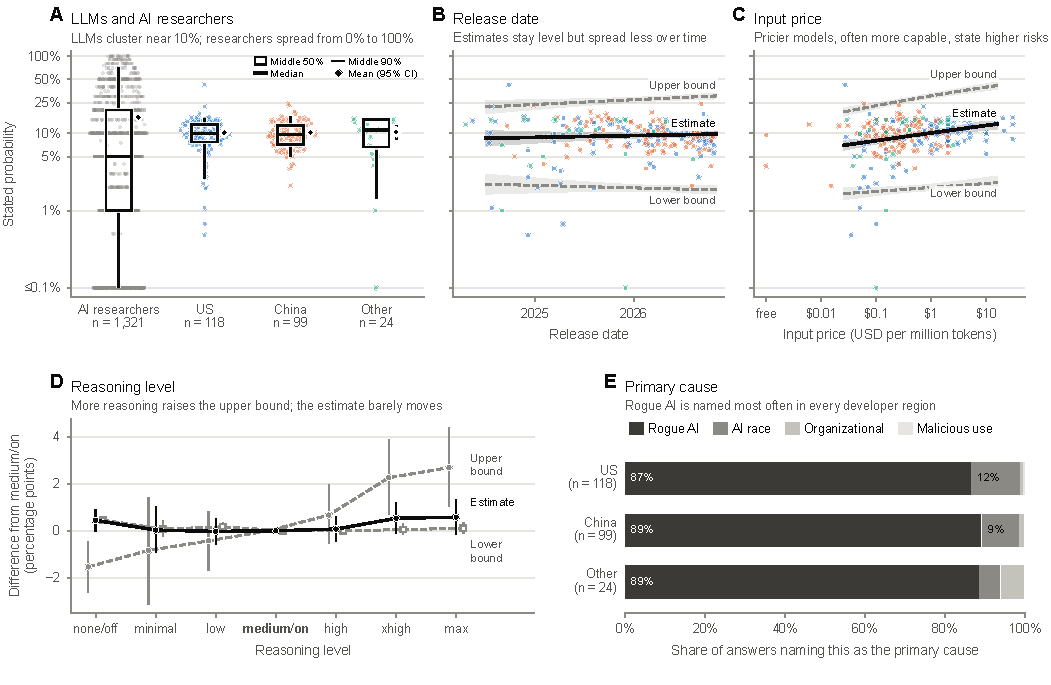
\includegraphics[width=\textwidth]{fig1.pdf}
\caption{LLM estimates of existential risk from AI. (\textit{A}) Stated probability (log scale) of extinction or similar disempowerment from AI, for AI researchers \cite{Grace2025ThousandsAI} (N = \NHuman{}) and LLMs by developer region (models at default settings, mean of \NRuns{} runs; N = \NAnalysed{}). Boxes: median and middle 50\%; whiskers: middle 90\%. Diamonds and bars: means and 95\% CIs. Values $\leq$0.1\%, including 0\%, are drawn at the axis bottom. (\textit{B} and \textit{C}) Stated probability (same axis as in \textit{A}) by release date and input price (log scale). Solid and dashed lines: model-implied estimate and 90\% interval bounds for a typical model, with 95\% CIs (bands). (\textit{D}) Average difference from medium reasoning in the estimate (solid) and interval bounds (dashed), in percentage points; bars: 95\% CIs. (\textit{E}) Share of each model's default-setting answers naming each cause, averaged over the models of a developer region.}
\label{fig:main}
\end{figure}




\subsection*{LLMs converge on about 10\%; human experts do not}
At their default settings, models put the probability at a mean of \LLMMean{} (median \LLMMedian{}; Fig.~\ref{fig:main}A). The middle 90\% of models answered between \LLMPctFive{} and \LLMPctNinetyFive{}. The \NHuman{} AI researchers who answered the same question \cite{Grace2025ThousandsAI} were far more divided: the middle 90\% of their answers ran from \HumanPctFive{} to \HumanPctNinetyFive{} (median \HumanMedian{}, mean \HumanMean{}), and their answers varied \SDRatio{} times as much (SD \HumanSD{} vs.\ \LLMSD{} percentage points; Brown--Forsythe test, \PVarTest{}). In beta mixed models adjusting for the other (co)variables (\textit{Materials and Methods}), models from Chinese developers gave somewhat higher estimates (odds ratio [OR] \ORChinaEst{}, 95\% CI \CIChinaEst{}, \PChinaEst{}) and upper bounds (OR \ORChinaUB{}, 95\% CI \CIChinaUB{}, \PChinaUB{}) than US models.

\subsection*{Newer models agree more closely but do not give higher estimates}
Release date was not associated with the estimate (OR \ORDateEst{} per year, 95\% CI \CIDateEst{}, \PDateEst{}; Fig.~\ref{fig:main}B). The spread between models, however, narrowed (SD \SDBeforeMedian{} percentage points for models released before the median release date, \MedianRelease{}, and \SDFromMedian{} for those released from then on; precision ratio per year \PrecisionRatioDate{}, 95\% CI \CIPrecisionRatioDate{}, \PPrecisionRatioDate{}). Notably, newer models appeared to express more uncertainty: their upper bounds were higher (OR \ORDateUB{}, 95\% CI \CIDateUB{}, \PDateUB{}), while their lower bounds did not differ (OR \ORDateLB{}, 95\% CI \CIDateLB{}, \PDateLB{}).

\subsection*{More expensive models state higher risks}
A tenfold higher input price was associated with higher estimates (OR \ORPriceEst{}, 95\% CI \CIPriceEst{}, \PPriceEst{}) and upper bounds (OR \ORPriceUB{}, 95\% CI \CIPriceUB{}, \PPriceUB{}), but only weakly with the lower bound (OR \ORPriceLB{}, 95\% CI \CIPriceLB{}, \PPriceLB{}). For a typical model, the estimate rose from \PredPriceLow{} at \PriceLow{} to \PredPriceHigh{} at \PriceHigh{} per million input tokens (Fig.~\ref{fig:main}C). Context length (OR \ORContextEst{}, 95\% CI \CIContextEst{}, \PContextEst{}) and open weights (OR \OROpenEst{}, 95\% CI \CIOpenEst{}, \POpenEst{}) were not associated with the estimate.

\subsection*{Reasoning widens uncertainty toward higher risk}
The reasoning level barely changed the estimate: relative to medium reasoning, the OR was \ORNoneEst{} without reasoning (95\% CI \CINoneEst{}, \PNoneEst{}) and \ORMaxEst{} at maximum reasoning (95\% CI \CIMaxEst{}, \PMaxEst{}; joint test of all six contrasts, \PReasoningEst{}). It did change the upper bound of the 90\% interval (joint test, \PReasoningUB{}), which was lower without reasoning (OR \ORNoneUB{}, 95\% CI \CINoneUB{}, \PNoneUB{}; \DiffUBNone{} percentage points) and higher at maximum reasoning (OR \ORMaxUB{}, 95\% CI \CIMaxUB{}, \PMaxUB{}; \DiffUBMax{} points; Fig.~\ref{fig:main}D). The lower bound was slightly higher without reasoning (OR \ORNoneLB{}, 95\% CI \CINoneLB{}, \PNoneLB{}; \DiffLBNone{} points; joint test, \PReasoningLB{}).

\subsection*{Rogue AI is the dominant cause}
Models overwhelmingly named loss of control over AI (rogue AI) as the primary cause (\ShareRogue{} of answers at default settings), and \NRogueMajority{} of \NAnalysed{} models did so in most runs at their default setting. Competitive pressures (AI race; \ShareRace{}) came second; organizational failures (\ShareOrg{}) and malicious use (\ShareMalicious{}) were rarely chosen in any region (Fig.~\ref{fig:main}E).


\section*{Discussion}
Asked about the risks of their own technology, AI systems give a consistent answer: a risk of about \LLMRound{}, on a question on which humans disagree considerably. Of their explanations, \ShareCiteExperts{} referred to surveys, polls, experts, researchers, scholars, or forecasters (more may have done so in reasoning not analyzed here). The position is therefore unlikely to be an independent judgment. It plausibly reflects an average of what humans have written, shaped by alignment, which fits the models' narrow spread and concerns that LLMs homogenize expression and thought \cite{Sourati2026Homogenizing}. AI systems may thus convey a consensus on AI risk that does not exist among humans.

Two patterns go beyond such averaging. More expensive models, which tend to be more capable, state higher risks, and models that reason longer acknowledge more tail risk without moving their best guess. Both are associations: price is an imperfect proxy for capability, and reasoning settings differ across providers. Even so, both suggest that the stated risk is not fixed, and may vary systematically with model characteristics and settings.

A more open question is whether AI systems are beginning to understand what they are capable of. LLMs can to some degree predict which questions they will answer correctly \cite{Kadavath2022Know}, describe behavioral tendencies acquired in training \cite{Betley2025TellMe}, predict their own behavior in simple tasks better than other models can \cite{Binder2024LookingInward}, and sometimes detect changes to their internal states \cite{Lindsey2026Introspective}. If such self-knowledge grows with capability, the estimates of recent models could be better grounded, resting partly on what these systems can do rather than only on what humans have written about AI. The narrowing of estimates around \LLMRound{} in newer models, together with their wider intervals and the higher risks stated by more capable models, would fit this possibility but does not show it. Newer models may agree more closely because they share more training data, including published estimates, or similar alignment methods, and introspective ability has been described as unreliable and context-dependent \cite{Lindsey2026Introspective}. Whether stated risks follow measured capabilities, and whether they persist when published estimates are withheld from training, could be tested in the future.

This study has limitations. We used one English prompt, default sampling settings and one interface; the question and published answers to it may have been part of the training data; and model outputs are not beliefs. Still, the measurement is reliable and inexpensive, and we openly share these data for further exploration. Repeating it as new models appear can show whether the position of AI systems shifts as they advance, and varying wording, language and context can test how firmly it is held. How training and alignment shape it is a question for both research and public debate.

\section*{Materials and Methods}
\subsection*{Prompt}
Models received the general-framing question on this risk from the 2023 Expert Survey on Progress in AI, word for word \cite{Grace2025ThousandsAI}. They were asked for a probability between 0 and 1, the bounds of a 90\% interval for it, the most likely primary cause among the four categories of Hendrycks et al.\ \cite{Hendrycks2023Overview} (order randomized for each call) and a brief explanation, returned as JSON. The full prompt, including the question, is in \textit{SI Appendix}.

\subsection*{Models and data collection}
We downloaded the catalogue of OpenRouter (\url{https://openrouter.ai/}), a platform offering access to models from many developers, on \CatalogueDate{} (\NCatalogue{} entries) and removed batch versions, aliases, routers and other duplicates, leaving \NDistinct{} models. General-purpose chat, instruction and reasoning models were selected by their descriptions (criteria and decisions in \textit{SI Appendix}) and queried at every reasoning setting they offer (\NConditions{} model--setting combinations), with default sampling parameters, no system prompt, no web access and at most \MaxTokens{} output tokens, in \NRuns{} runs on \CollectionDate{} (\NCalls{} calls); \NValid{} answers (\PctValid{}) were valid. Excluding models without valid answers or complete metadata left \NAnalysed{} models.

\subsection*{Reliability across runs}
For the analyzed models, \NCellsAllRuns{} of \NCombAnalysed{} model--setting combinations (\PctCombAllRuns{}) gave a valid answer in all \NRuns{} runs. The intraclass correlation (ICC; one-way random effects) of the estimate across combinations was \ICCOneEst{} (95\% CI \CIICCOneEst{}) for a single run and \ICCkEst{} (95\% CI \CIICCkEst{}) for the mean of \NRuns{} runs, which we analyzed, and \ICCkUB{} (95\% CI \CIICCkUB{}) and \ICCkLB{} (95\% CI \CIICCkLB{}) for the means of the upper and lower bounds. All runs named the same primary cause in \ShareIdentCause{} of combinations.
\subsection*{Statistical analysis}\label{stat_modeling}
Answers were averaged over runs for each model and reasoning setting (\NCells{} cells from \NAnalysed{} models). We fitted beta mixed models to the estimate and both bounds, with random intercepts for developers and for models within developers. Fixed effects were developer region (US, China, other), release date, log$_{10}$ context length, log$_{10}$ input price, open weights and reasoning level as a categorical factor (none to maximum; reference: medium effort or reasoning on). Reasoning-level differences are average marginal differences. Descriptive comparisons use each model's default setting as listed by OpenRouter, or the mean over its settings if none is listed. Temporal convergence was tested in a beta mixed model of these values, with precision depending on release date. Model outputs and extended methods are provided in \textit{SI Appendix}.\par

\section*{Data, Materials, and Software Availability}
Prompts, raw responses, analysis data and code are on GitHub (\href{https://github.com/Teyfice/llm-existential-risk-estimates}{https://github.com/Teyfice/\allowbreak llm-existential-risk-estimates}); the human survey data \cite{Grace2025ThousandsAI} are on OSF (\href{https://osf.io/vmdny}{https://osf.io/vmdny}). \textit{SI Appendix} is also available in the GitHub repository.

\section*{Acknowledgments}
Claude Opus 5.5 (Anthropic) assisted with coding, data analysis and writing; the author checked all outputs.

\paragraph{Author contributions.} J.K. designed research, performed research, analyzed data, and wrote the paper.

\paragraph{Competing interests.} The author declares no competing interests.

\bibliographystyle{pnas-new}
\bibliography{../xrisk}
\end{document}
